\section{Diseño}

%Normal Slide (copy, paste and modify this slide for longer presentations)
\begin{frame}
\frametitle{\secname} %Title
\framesubtitle{Arquitectura} %Subtitle
\rmfamily %Font
\color{black} %Color
\begin{itemize}
    \item \rojoUMU{Arquitectura} propuesta.
\begin{figure}
    \centering
    \resizebox{0.8\textwidth}{!}{
        \begin{tikzpicture}
    % Cajas grandes
    \node[draw, rounded corners, minimum width=6cm, minimum height=8cm, fill=yellow!20] (0) {};
    \node (1) [above = 0cm of 0] {Dispositivo IoT};
    \node[draw, rounded corners, minimum width=6cm, minimum height=8cm, fill=red!20] (2) [right = of 0] {};
    \node (3) [above = 0cm of 2] {Cliente externo};
    
    % Parte IoT
    \node[draw, rounded corners, minimum width=5cm, fill=gray!10, text width=4.5cm, align=flush center, font=\scriptsize] (4) at ($(0) + (0, 2)$) {A. Establecimiento de las condiciones};
    \node[draw, rounded corners, minimum width=5cm, fill=yellow!5, text width=4.5cm, align=left, font=\scriptsize] (5) [below = 0cm of 4] {- Establecer una frecuencia fija. \\ - Desactivar servicio NTP.};
    
    \node[draw, rounded corners, minimum width=5cm, fill=gray!10, text width=4.5cm, align=flush center, font=\scriptsize] (6) at ($(0) + (0, -1)$) {B. Recolección de datos};
    \node[draw, rounded corners, minimum width=5cm, fill=yellow!5, text width=4.5cm, align=left, font=\scriptsize] (7) [below = 0cm of 6] {- Obtener marcas de tiempo. \\ - Enviar el dato al cliente.};
    
    % Parte externa
    \node[draw, rounded corners, minimum width=5cm, fill=gray!10, text width=4.5cm, align=flush center, font=\scriptsize] (8) at ($(2) + (0, 3)$) {C. Análisis y procesamiento de los datos};
    \node[draw, rounded corners, minimum width=5cm, fill=red!5, text width=4.5cm, align=left, font=\scriptsize] (9) [below = 0cm of 8] {- Obtener incremento respecto al dato anterior. \\ - Generación de estadísticas. \\ - Reducción de dimensionalidad.};
    
    \node[draw, rounded corners, minimum width=5cm, fill=gray!10, text width=4.5cm, align=flush center, font=\scriptsize] (10) at ($(2) + (0, 0.4)$) {D. Generación de los modelos};
    \node[draw, rounded corners, minimum width=5cm, fill=red!5, text width=4.5cm, align=left, font=\scriptsize] (11) [below = 0cm of 10] {- Elegir los algoritmos de CL$^1$ / DA$^2$. \\ - Ajustar hiperparámetros y generar el modelo.};
    
    \node[draw, rounded corners, minimum width=5cm, fill=gray!10, text width=4.5cm, align=flush center, font=\scriptsize] (12) at ($(2) + (0, -2)$) {E. Evaluación de los modelos};
    \node[draw, rounded corners, minimum width=5cm, fill=red!5, text width=4.5cm, align=left, font=\scriptsize] (13) [below = 0cm of 12] {- Elección de métricas. \\ - Evaluación de los modelos. \\ - Comparar métricas};
    
    
    % Aclaraciones
    \node[minimum width=6cm, text width=5.2cm, align=left, font=\scriptsize] (14) [below = 0cm of 2] {1: Clasificación \\ 2: Detección de anomalías};
    
    % Iconos
    \node (15) at ($(0.north east) + (-0.5, 0)$) {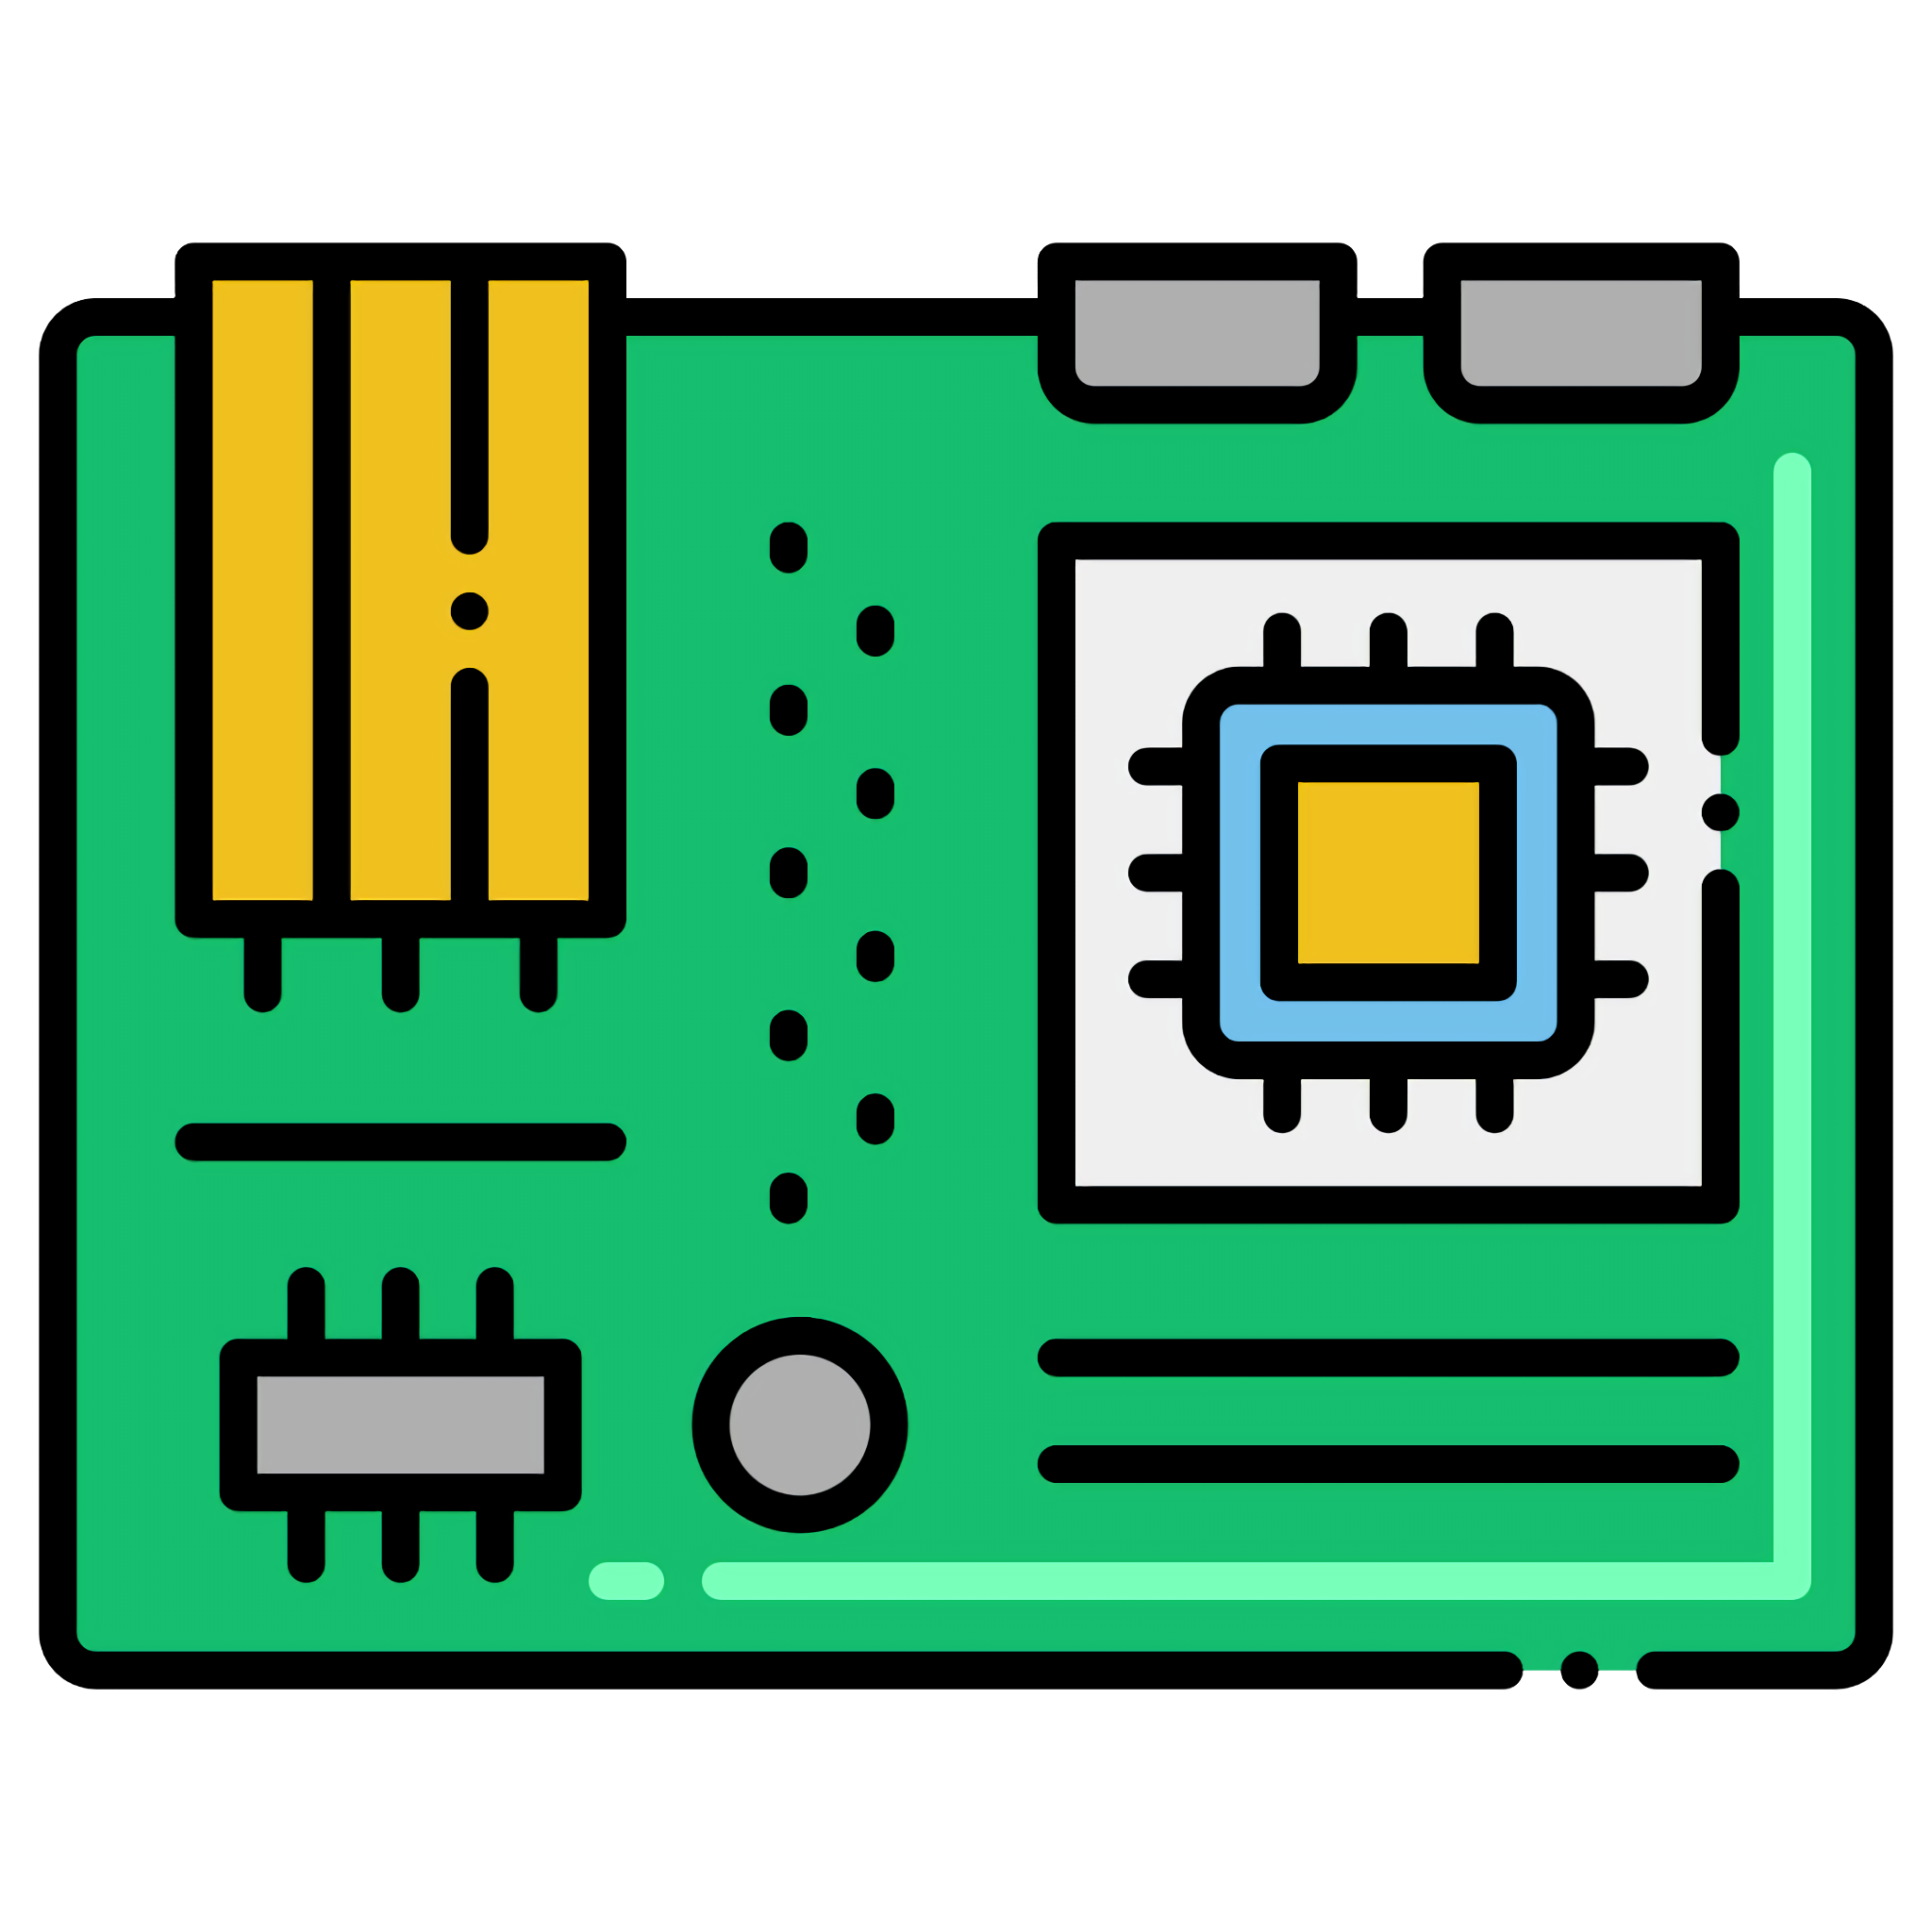
\includegraphics[scale=0.08]{images/board.png}};
    \node (16) at ($(2.north east) + (-0.5, 0.1)$) {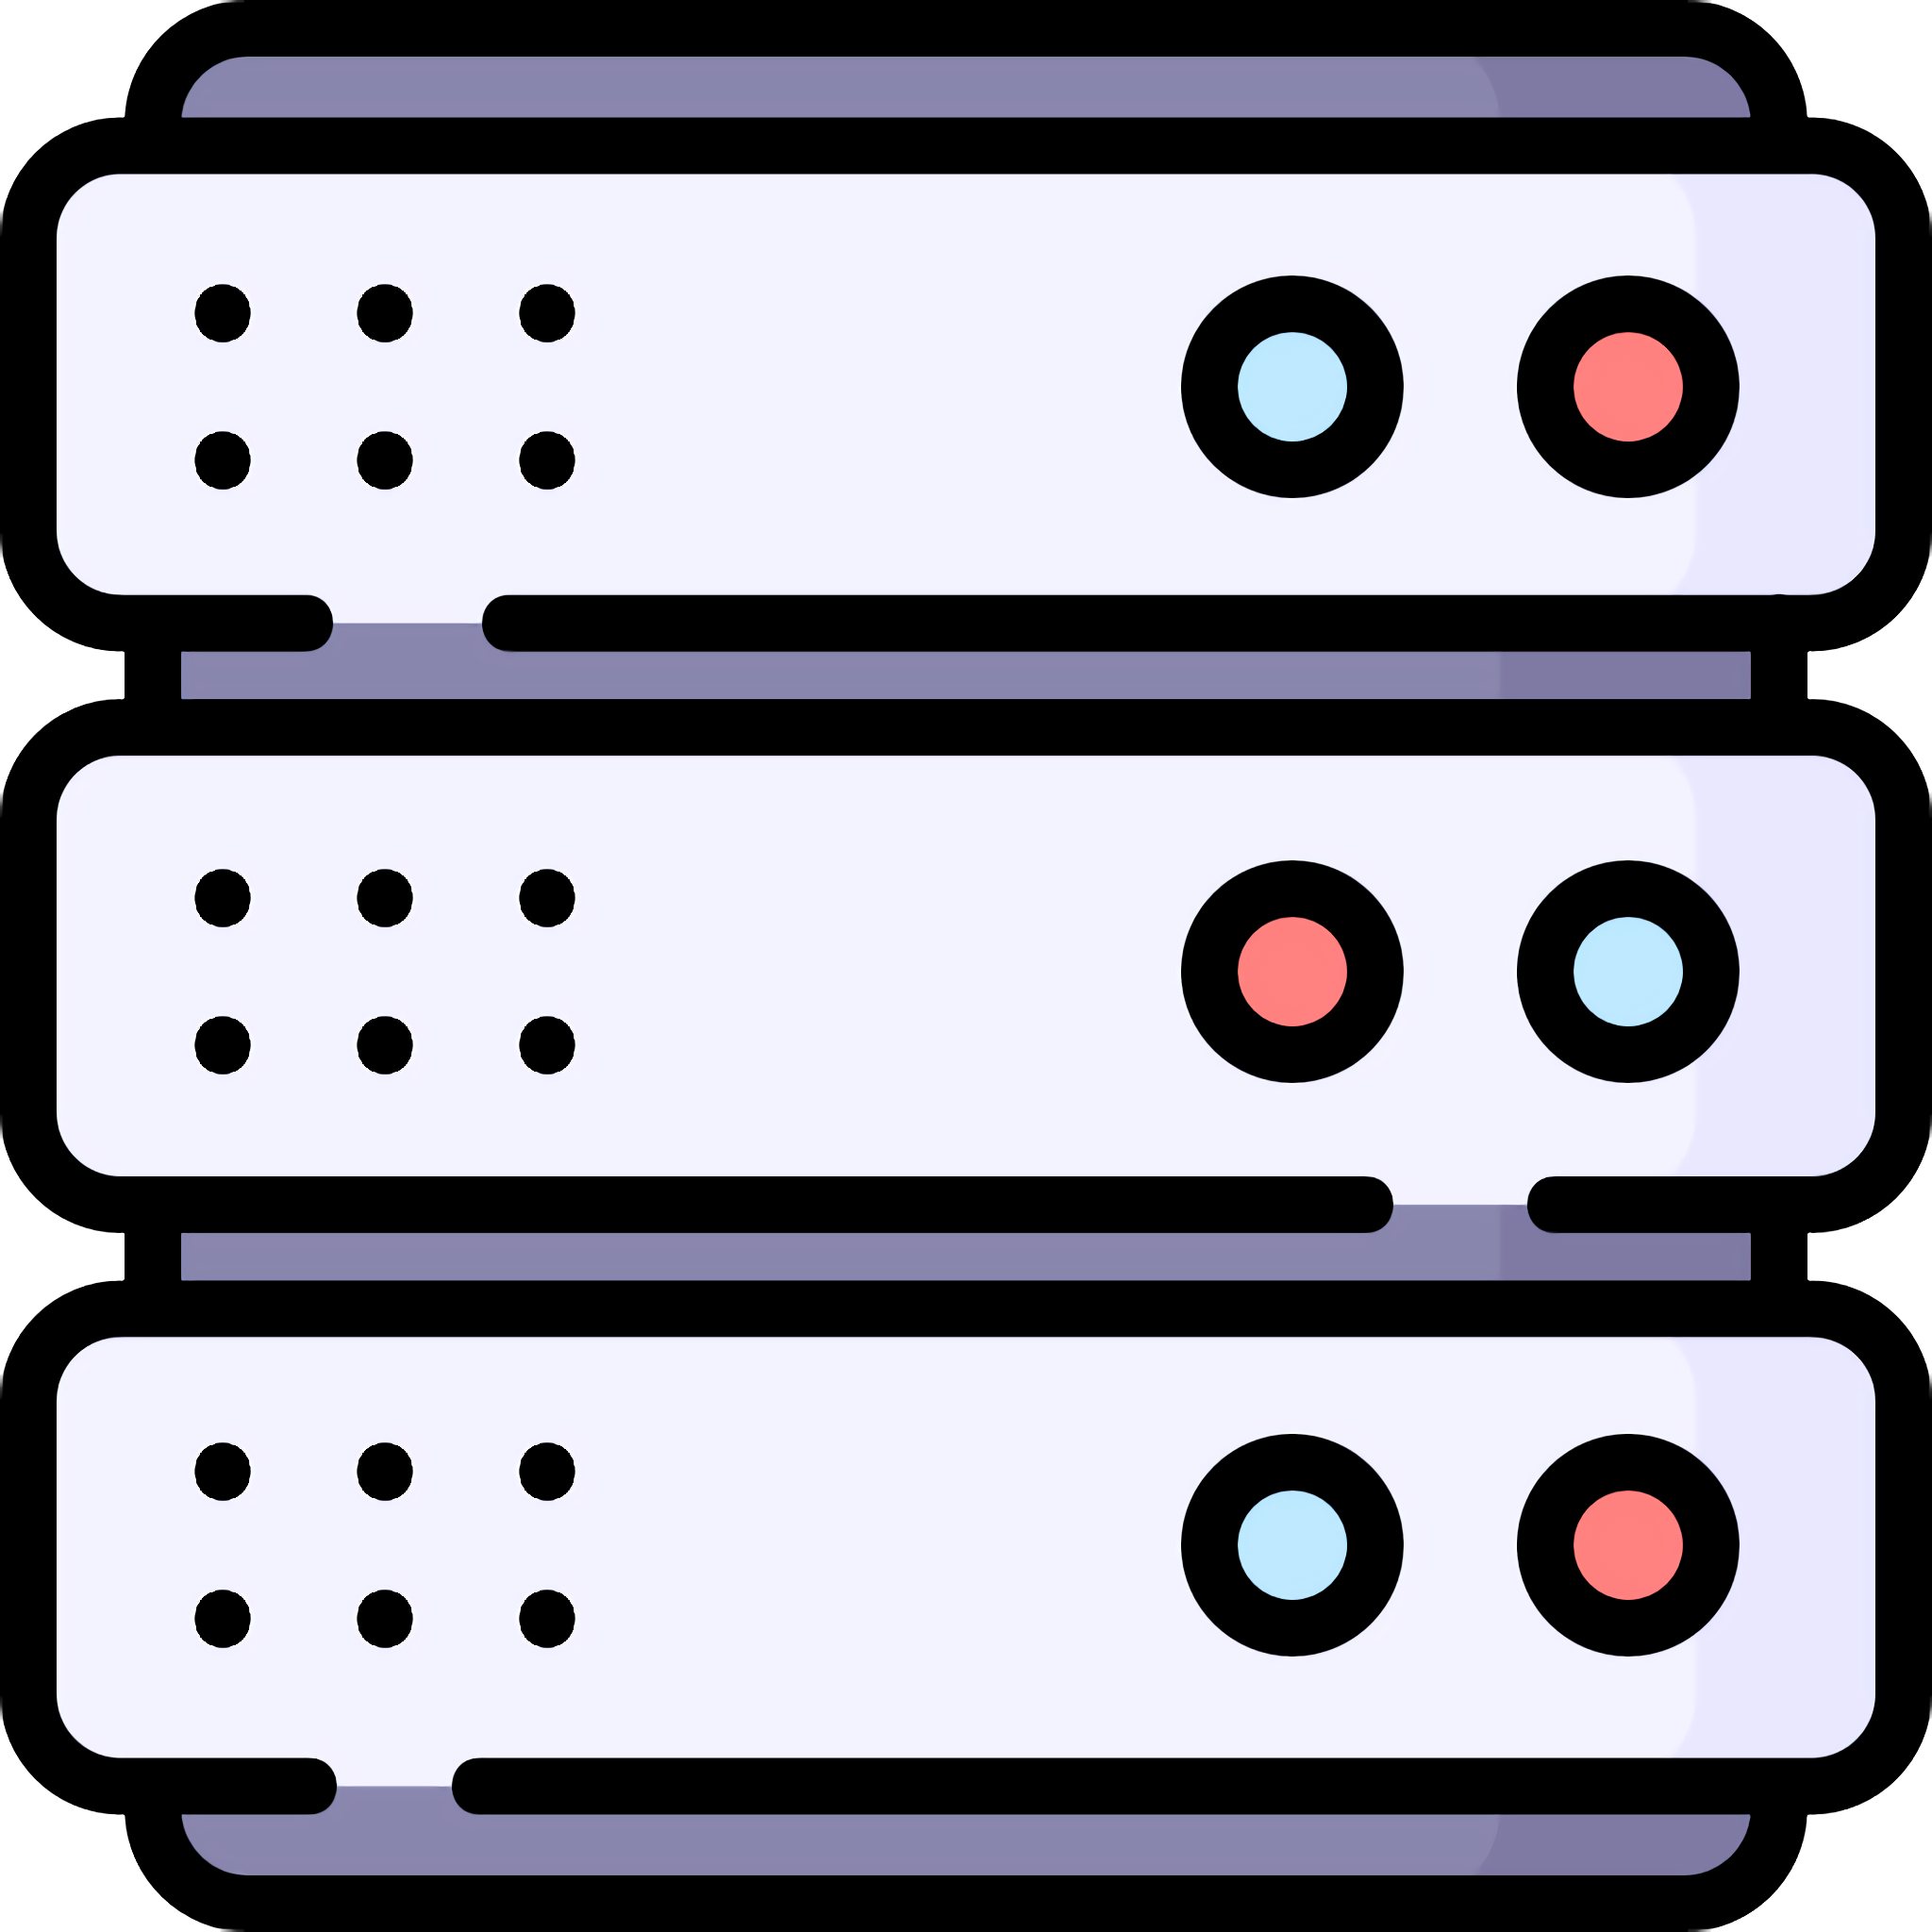
\includegraphics[scale=0.07]{images/server.png}};
    
    \draw (5) -- (6);
    \draw[rounded corners] ($(7.north west) - (0, 0.15)$) -| ++(-0.3, -0.268) |- ($(7.south west) + (0, 0.15)$);
    \draw[rounded corners] (7.east) -| ++(1,0) |- (9.west);
    \draw (9) -- (10);
    \draw (11) -- (12);
 \end{tikzpicture}
    }
\end{figure}
\end{itemize}
\end{frame}

%Normal Slide (copy, paste and modify this slide for longer presentations)
\begin{frame}
\frametitle{\secname} %Title
\framesubtitle{Topología} %Subtitle
\rmfamily %Font
\color{black} %Color
\begin{itemize}
    \item \rojoUMU{Topología} de la red.
\begin{figure}
    \centering
    \resizebox{0.8\textwidth}{!}{
        \begin{tikzpicture}
    \node (1) {
\includegraphics{cisco_icons/cloud}};
    \node (2) [below = of 1] {
\includegraphics{cisco_icons/router}};
    \node (3) [below = of 2] {$\substack{
\includegraphics{cisco_icons/pc} \\ \text{Observador}}$};
    \node (aux) [below =0.4cm of 3] {};
    \node (4) [below = of aux] {$\substack{
\includegraphics{cisco_icons/pc} \\ \text{Disp. 3}}$};
    \node (5) [left = of 4] {$\substack{
\includegraphics{cisco_icons/pc} \\ \text{Disp. 2}}$};
    \node (6) [left = of 5] {$\substack{
\includegraphics{cisco_icons/pc} \\ \text{Disp. 1}}$};
    \node (7) [right = of 4] {$\substack{
\includegraphics{cisco_icons/pc} \\ \text{Disp. 4}}$};
    \node (8) [right = of 7] {$\substack{
\includegraphics{cisco_icons/pc} \\ \text{Disp. 5}}$};
    \node (text) {Internet};
    \draw[-] (1) -- (2); 
    \draw[-] (2) -- (3);
    \draw[-] (3) -- (4);
    \draw[-] (aux.center) -| (6);
    \draw[-] (aux.center) -| (5);
    \draw[-] (aux.center) -| (7);
    \draw[-] (aux.center) -| (8);
\end{tikzpicture}
    }
\end{figure}
\end{itemize}
\end{frame}

%Normal Slide (copy, paste and modify this slide for longer presentations)
\begin{frame}
\frametitle{\secname} %Title
\framesubtitle{Recolección de datos} %Subtitle
\rmfamily %Font
\color{black} %Color
\begin{minipage}{0.5\textwidth}
\begin{itemize}
    \item La marca de tiempo relativa a cada mensaje desde el inicio, \rojoUMU{$t_i - t_{start}$}.
    \item La marca de tiempo absoluta del observador \rojoUMU{$t_i$}.
    \item La marca de tiempo absoluta del dispositivo \rojoUMU{$t'_i$}.
    \item La desviación del reloj del dispositivo respecto al del observador, \rojoUMU{$t_i - t'_i$}.
\end{itemize}
\end{minipage}
\begin{minipage}{0.3\textwidth}
\begin{figure}
    \centering
    \resizebox{1.7\textwidth}{!}{
    \begin{sequencediagram}
        \newthread{o}{Observador}
        \newinst[3]{d}{Dispositivo $x$}
        
        \begin{call}{o}{Obtener marca de tiempo}{o}{$t_i$}
        \end{call}
        
        \postlevel
        
        \begin{call}{o}{Obtener tiempo relativo al mensaje}{o}{$t_i - t_{start} \approx i$}
        \end{call}
        
        \postlevel
        
        \begin{call}{o}{Pedir marca de tiempo}{d}{Devolver $t'_i$}
        \end{call}
        
        \postlevel
        
        \begin{call}{o}{Obtener desviación}{o}{$t_i - t'_i$}
        \end{call}
    \end{sequencediagram}
    }
\end{figure}
\end{minipage}
\end{frame}

%Normal Slide (copy, paste and modify this slide for longer presentations)
\begin{frame}
\frametitle{\secname} %Title
\framesubtitle{Evaluación de los resultados} %Subtitle
\rmfamily %Font
\color{black} %Color
\begin{itemize}
    \item Evaluación de los resultados.
        \begin{itemize}
            \item Algoritmos de ML supervisados para \rojoUMU{clasificación}.
            \item Algoritmos de ML no supervisados para \rojoUMU{detección de anomalías}.
        \end{itemize}
\end{itemize}
{\small
\begin{multicols}{2}
\begin{equation*}
    Accuracy = \frac{TP + TN}{TP + FP + FN + TN}
\end{equation*}
\begin{equation*}
    Recall = \frac{TP}{TP + FN}
\end{equation*}
\begin{equation*}
    f-score = \frac{2 \cdot TP}{2 \cdot TP + FP + FN}
\end{equation*}
\begin{equation*}
    TNR = \frac{TN}{TN + FP}
\end{equation*}
\end{multicols}
}
\end{frame}





